% !TEX TS-program = pdflatex
% !TEX encoding = UTF-8 Unicode

% This is a simple template for a LaTeX document using the "article" class.
% See "book", "report", "letter" for other types of document.

\documentclass[11pt]{article} % use larger type; default would be 10pt

\usepackage[utf8]{inputenc} % set input encoding (not needed with XeLaTeX)
\usepackage{graphicx}
\usepackage{algorithm}
\usepackage{algorithmicx}
\usepackage{algpseudocode}
\usepackage{multirow}

%%% Examples of Article customizations
% These packages are optional, depending whether you want the features they provide.
% See the LaTeX Companion or other references for full information.

%%% PAGE DIMENSIONS
\usepackage{geometry} % to change the page dimensions
\geometry{a4paper} % or letterpaper (US) or a5paper or....
% \geometry{margin=2in} % for example, change the margins to 2 inches all round
% \geometry{landscape} % set up the page for landscape
%   read geometry.pdf for detailed page layout information

\usepackage{graphicx} % support the \includegraphics command and options

% \usepackage[parfill]{parskip} % Activate to begin paragraphs with an empty line rather than an indent

%%% PACKAGES
\usepackage{booktabs} % for much better looking tables
\usepackage{array} % for better arrays (eg matrices) in maths
\usepackage{paralist} % very flexible & customisable lists (eg. enumerate/itemize, etc.)
\usepackage{verbatim} % adds environment for commenting out blocks of text & for better verbatim
\usepackage{subfig} % make it possible to include more than one captioned figure/table in a single float
% These packages are all incorporated in the memoir class to one degree or another...

%%% HEADERS & FOOTERS
\usepackage{fancyhdr} % This should be set AFTER setting up the page geometry
\pagestyle{fancy} % options: empty , plain , fancy
\renewcommand{\headrulewidth}{0pt} % customise the layout...
\lhead{}\chead{}\rhead{}
\lfoot{}\cfoot{\thepage}\rfoot{}

%%% SECTION TITLE APPEARANCE
\usepackage{sectsty}
\allsectionsfont{\sffamily\mdseries\upshape} % (See the fntguide.pdf for font help)
% (This matches ConTeXt defaults)

%%% ToC (table of contents) APPEARANCE
\usepackage[nottoc,notlof,notlot]{tocbibind} % Put the bibliography in the ToC
\usepackage[titles,subfigure]{tocloft} % Alter the style of the Table of Contents
\renewcommand{\cftsecfont}{\rmfamily\mdseries\upshape}
\renewcommand{\cftsecpagefont}{\rmfamily\mdseries\upshape} % No bold!

%%% END Article customizations

%%% The "real" document content comes below...

\title{Lab 7: Search and Retrieval}
\author{Ruofan Zhou}
%\date{} % Activate to display a given date or no date (if empty),
         % otherwise the current date is printed 

\begin{document}
\maketitle

\section{VSM}
\subsection{
20 search results for the query "James Bond 007": }
\tiny
01. Dr. No (1962) (score: 0.97655) \\
02. James Bond: Shaken and Stirred (1997) (TV) (score: 0.93868) \\
03. Casino Royale (1967) (score: 0.88774) \\
04. The World Is Not Enough (1999) (score: 0.76798)\\
05. The Living Daylights (1987) (score: 0.74025)\\
06. Die Another Day (2002) (score: 0.73592)\\
07. The Making of 'The World Is Not Enough' (1999) (V) (score: 0.70328)\\
08. Zero Posterity (2006) (V) (score: 0.68285)\\
09. On Her Majesty's Secret Service (1969) (score: 0.68193)\\
10. Licence to Kill (1989) (score: 0.66520)\\
11. True Bond (2007) (TV) (score: 0.66456)\\
12. The Goldfinger Phenomenon (1995) (V) (score: 0.66218)\\
13. James Bond: Licence to Thrill (1987) (TV) (score: 0.64977)\\
14. Ian Fleming on Desert Island Discs (2006) (V) (score: 0.64037)\\
15. Never Say Never Again (1983) (score: 0.63990)\\
16. Donna James \& Gary (2006) (score: 0.62717)\\
17. Tomorrow Never Dies (1997) (score: 0.61642)\\
18. The Last Call (2012/I) (score: 0.61544)\\
19. Live and Let Die (1973) (score: 0.61257)\\
20. La faute des autres (1923) (score: 0.59509)\\
\normalsize
\subsection{
20 search results for the query Internet Analytics course description and explaination for "Babe(1981)" has a high ranking. }\\
\tiny
01. Paintbrush (2008) (score: 1.12490)\\
02. Babe (1981) (score: 0.97120)\\
03. Have I Shared Too Much? (2011) (score: 0.96333)\\
04. Eu Odeio o Orkut (2011) (score: 0.82655)\\
05. I Love Alaska (2009) (score: 0.81054)\\
06. Death Drives a Wheelchair (2011) (score: 0.80866)\\
07. The First Measured Century (2000) (TV) (score: 0.79080)\\
08. System of Units (2004) (score: 0.77668)\\
09. Caught in the Web (2012) (score: 0.73015)\\
10. Ladybird Ladybird (1994) (score: 0.71697)\\
11. IRL (In Real Life) (2007) (V) (score: 0.70784)\\
12. Koleksiyoncu: The Collector (2002) (score: 0.70378)\\
13. "The Onion's Extremely Accurate History of the Internet" (2012) (score: 0.69442)\\
14. War for the Web (2014) (score: 0.68898)\\
15. Code Red: China's Cyber Civil War (2012) (score: 0.68012)\\
16. Student Loans (2001) (V) (score: 0.67663)\\
17. Regards croisés (2009) (V) (score: 0.67580)\\
18. World Wide Dead (2008) (score: 0.67272)\\
19. When Hunky Met Dory (2011) (score: 0.67209)\\
20. Modele (2009) (TV) (score: 0.66905)\\
\normalsize
\\
For "Babe(1981)", we can find its plot as below:\\
\\
\emph{
030873	One thing stands between a successful model and a multi-million dollar inheritance: she has to be married to collect! She searches for Mr. Right, a guy interested ONLY as a business partner so she can quit working. Meanwhile, her modeling agent searches for Mr. Wrong, so as not to lose her agency's top model. They meet in the middle - with surprising results!}\\ \\
We can find that there are some keyword like \emph{model}, \emph{collect} and \emph{search} also appear in the course descprition. And since these words may not often appear in other movies' plots so they weights much thus made the movie have a high ranking.

\section{LSI}
\subsection{20 search results for the query "James Bond 007"}
\tiny
01. La faute des autres (1923) (score: 0.37510)\\
02. The Last Call (2012/I) (score: 0.37391)\\
03. True Bond (2007) (TV) (score: 0.37150)\\
04. Donna James \& Gary (2006) (score: 0.36590)\\
05. Beyond Loch Ness (2008) (TV) (score: 0.36065)\\
06. One Goal, One Hope (2010) (score: 0.36062)\\
07. On/Off (2003) (score: 0.35722)\\
08. Resonance (2011) (score: 0.35111)\\
09. A Boost of Love (2012) (score: 0.34914)\\
10. Crystal Jam (2010) (score: 0.34275)\\
11. Ratcatcher (1999) (score: 0.34053)\\
12. Casino Royale (1967) (score: 0.34008)\\
13. Massa'ot James Be'eretz Hakodesh (2003) (score: 0.33933)\\
14. James (2008) (score: 0.33534)\\
15. On Her Majesty's Secret Service (1969) (score: 0.33304)\\
16. The Pursuit (2008/I) (score: 0.33195)\\
17. James Bond: Licence to Thrill (1987) (TV) (score: 0.33062)\\
18. Erotic Obsessions (2002) (V) (score: 0.32966)\\
19. Down the Coast (2011) (score: 0.32904)\\
20. Ghost Soldier (2006) (score: 0.32773)\\
\normalsize

\subsection{The terms that have extremal values along the first dimension uncovered by the SVD}
dimension 1 - terms with lowest values:\\
bathi birodalmaiban hazajaban irodalmar kalandjat kepzelet legkulonosebb tudomani londonban misztikum nazzaro martoni licli lectual suspi standabl horri pointment onstrat gler enc cial cion canniti benefi celebra boarderless antiqui sadduce kerkerinck trutelink korteboldt lambertikirch prescib prinzipalmarkt osnabruck 1530s aquina unboyish ungrac vassilova nomic rangnagar pathless villagairosa sherdeman gainsvil 29s liebenberg peddlar \\
\\
dimension 1 - terms with highest values:\\
follow back first want own while wife how help where mother meet go us wai home peopl show you becom come t through work old woman dai father make time girl take what them friend two world year new famili get stori live young find love man film life him \\
\\ 
\section{pLSI}
\subsection{Plot of the log-likelihood at each iteration}
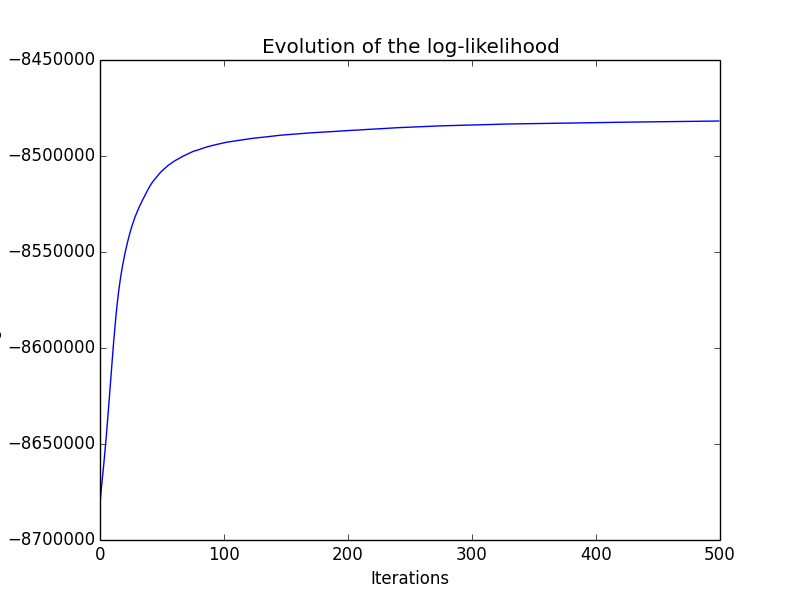
\includegraphics[width=13cm]{output/loglikelihood}
\\
500 iterations are enough since the log-likelihood doesn't change much after 350+ iterations.\\
The way to be sure the algorithm has converged is to set a maximum delta for log-likelihood between 2 iterations.\\
\subsection{Top 20 words for each topic}
topic 000: percent said million year market price new trade compani billion stock rate dollar down bank report share increas cent sale\\ \\
topic 001: said polic two peopl year kill charg fire report offic citi state offici arrest three dai mile court death prison\\ \\
topic 002: said i t year you new bush peopl dukaki go time school what presid do campaign dai get like work\\ \\
topic 003: said state year feder hous court new us senat bill plan program t d presid depart administr time govern case\\ \\
topic 004: said soviet govern u state presid parti offici unit nation new countri leader report year militari forc minist peopl union\\
\subsection{Latent meaning of each one of the topics}
topic 000: \textbf{economy} \\
topic 001: \textbf{justice} \\
topic 002: \textbf{life} \\
topic 003: \textbf{career} \\
topic 004: \textbf{high level} \\
\subsection{A way of adapting the clustering algorithm of the previous lab to automatically cluster
documents based on their topic distribution}
Using TF-IDF-weighted vectors and cosine similarity.
\end{document}
